\chapter{Results}

\section{ Answer to RQ1 : The computer simulation resemble experimental results of animal study}

\subsection{ The single cell properties of computational model and the whole cell patch clamp recording shows the same behavior}

Figure .1.1: Comparing the sample membrane potential trace of WT and KO during hyperpolarize current injection and depolarize current injection

Figure .1.2: Comparing the number of bursting spikes and tonic spikes between the simulated cell and experimental data


\subsection{  The cell population properties of computational model and the MUA cells recording shows the same behavior}

Figure .1.3 : Comparison of mean and standard deviation of observed firing rate in cell population in computational model and experimental data


\subsection{ Neuron activities during light-off period (no photoactivation)}

Figure .1.4 The baseline activities of neural population during light-off period show no significant different between WT and KO


\subsection{ Neuron activities during photoactivation}

Figure .1.5 The delay and peak of rebound spiking activity of WT and KO are significantly different. The WT shows short rebounding period and higher peak of neural activities


\subsection{ The coherence between VL and M1 layer shows that correlated neural activities after photoactivation ( the rebound bursting spikes) drives activity in M1}

Figure~\ref{fig:sample} The coherence between VL’s MUA and M1’s LFP

\begin{figure}
	\centering
	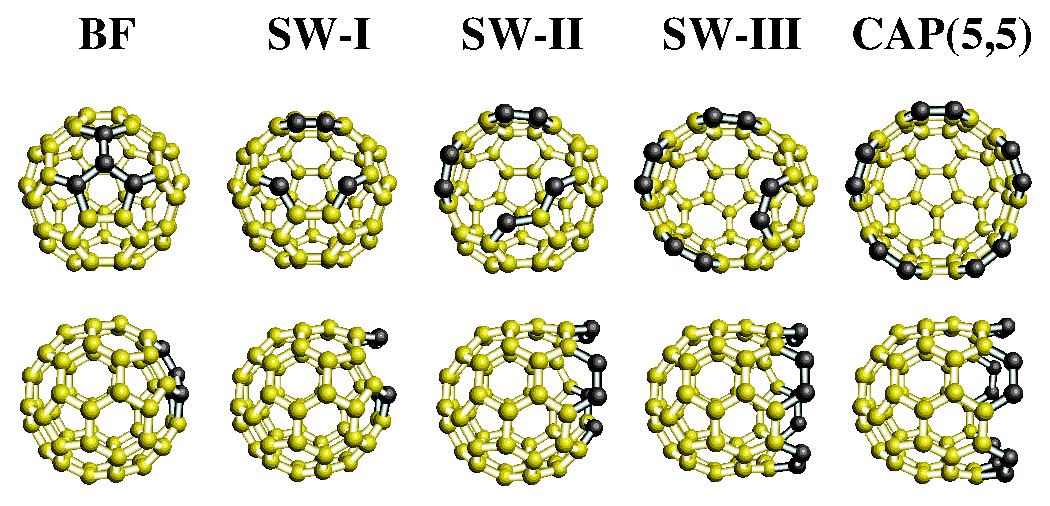
\includegraphics[width=0.5\textwidth]{figures/sample-fig1}
	\label{fig:sample}
	\caption{Sample Figure}
\end{figure}

\section{Answer to RG2 : Computational simulation predicts causal relationship of exceed motor command in M1 from VL in Parkinson’s disease patient}

\subsection{ The high synchronization (correlated neural activities) in VL but not average firing rate can drive M1’s motor command}


Figure .2.1 The high synchronized neural activities during bursting can drive M1 in WT types but not KO, even though the average firing rate if WT and KO are not significantly difference


\subsection{  The high synchronization level can be achieved by bursting. The demolishing of bursting in WT neurons result in the absent of synchronization in neuron population}

Figure .2.2 Schematic diagram of how the bursting activity cause high synchronization in neuron population

\subsection{ The Analysis of information transfer from VL to M1 : The information in VL can transfer to M1 when the neuron population in VL are synchronized }

Figure .2.3 the neural information from VL is transferring to M1 only when the neural activities in VL are synchronized.

Figure .2.4 the level of information transfer between VL and M1 is proportionally to the synchronization level in VL

\subsection{ Artificially generated bursting in KO neurons result in high synchronization level of neuron population which can drive M1’s motor command
}
Figure .2.5 successfully generated bursting behavior in KO with similar bursting behavior generated by T-Type Calcium channel in WT

Figure .2.6 The artificial bursting behavior in KO result in high level synchronization level of neural population and this high synchronized neural 
population can drive M1

\subsection{ Artificially activated VL neural population in theta and beta frequencies result in motor command from M1with the same frequency band with what observed in Parkinson’s disease patient.}

